\documentclass[10pt]{beamer}

\usepackage{silence}
\WarningFilter{biblatex}{File 'ngerman-iso.lbx'}

\usetheme{metropolis}
\usepackage{appendixnumberbeamer}
\usepackage{tabularx}


\usepackage[english,ngerman]{babel}
\graphicspath{ {./images} }
\usepackage{float,xcolor,csquotes,etoolbox}

\usepackage{hyperref}
\hypersetup{breaklinks,colorlinks,linkcolor=black,citecolor=black,filecolor=black,urlcolor=black}
\newcommand\urls[1]{%
  \href{https://#1}{\nolinkurl{#1}}%
}

\usepackage{tikz}
\usetikzlibrary{babel}


\usepackage[inkscapeformat=png,inkscapedpi=600]{svg}

\usepackage{xspace}
\usepackage{qrcode}

\qrset{level=H,hyperlink}

\setlength {\marginparwidth}{2cm}

\setbeamertemplate{frame footer}{%
    \hyperlink{unpuenktlich}{\beamergotobutton{Unpünktlich?}}
}

\title{Ersti-Begrüßung: Sommer Semester 26}
\subtitle{IT Setup}
\date{\today}
\author{Max Trautwein}
\institute{Fachschaft IT}

\begin{document}

\maketitle

\begin{frame}{Gliederung}
  \setbeamertemplate{section in toc}[sections numbered]
  \tableofcontents[hideallsubsections] %
\end{frame}

\section{Anfordeungn}

\begin{frame}{Anfordeungn} 
    \begin{itemize}
        \item HS Account
        \item Handy / Tablet (WLAN \& Mail)
        \item Laptop (WLAN, Mail, VPN)
    \end{itemize}
\end{frame}

\section{WLAN}

\begin{frame}{WLAN: 1. Login easyroam} 
    \begin{minipage} [t] {0.4\textwidth} 
      \qrcode[height=10em]{https://www.easyroam.de/}
        \\~\\~
        \Large
        \urls{www.easyroam.de}
    \end{minipage}
    \begin{minipage} [t] {0.4\textwidth}
     ~ 
    \end{minipage}

    \begin{tikzpicture}[remember picture, overlay]
        \node at ([yshift=2cm,xshift=-4cm]current page.east) {
            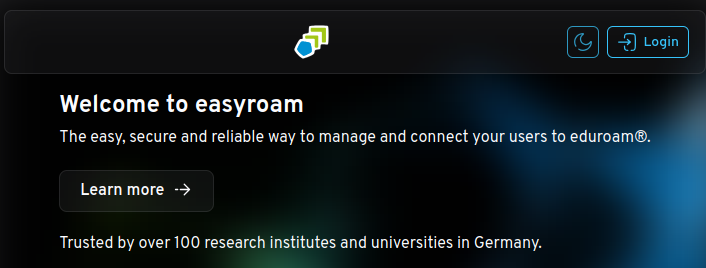
\includegraphics[width=6cm]{easyhome.png}
        };
        \draw[red, ultra thick] (9.9,5) rectangle (10.73,5.4);
        \node at ([yshift=-1cm,xshift=-4cm]current page.east) {
            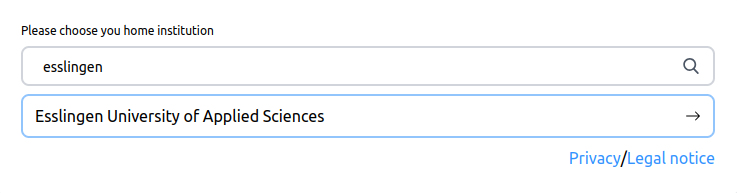
\includegraphics[width=6cm]{selecths.png}
        };
    \end{tikzpicture}
\end{frame}

\begin{frame}{WLAN: 2. DL \& Setup}

    \begin{tikzpicture}[remember picture, overlay]
        \node at ([yshift=0cm,xshift=3.5cm]current page.west) {
            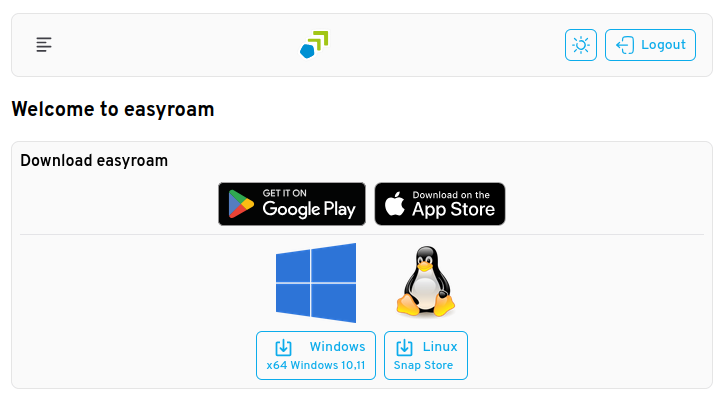
\includegraphics[width=6cm]{easyweb.png}
        };
        \node at ([yshift=0cm,xshift=-3.5cm]current page.east) {
            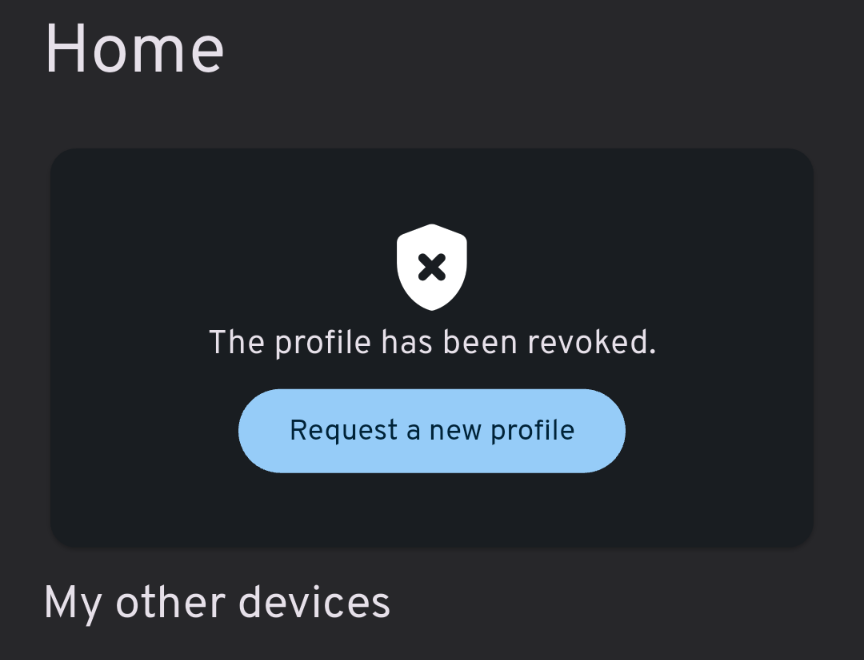
\includegraphics[width=5cm]{easyapp.png}
        };
        \draw[red, ultra thick] (7,-0.65) rectangle ++(2.6cm,.8cm);
    \end{tikzpicture}

\end{frame}

\section{Mail}

\begin{frame}{Mail}

\end{frame}

\section{VPN}

\begin{frame}{VPN}

\end{frame}


\begin{frame}[standout]
  Fragen?
\end{frame}

{
    \setbeamertemplate{frame footer}{}

    \begin{frame}[label=unpuenktlich]{Unpünktlich?}
        \centering\Large
        Slides:\\~\\
        \qrcode[height=13em,nolink]{https://www.bwsyncandshare.kit.edu/s/TGkjG9pxERRgmZo}
    \end{frame}
}



\end{document}